\documentclass{beamer}
\usepackage{xcolor} 
\usepackage[utf8]{inputenc}
\usetheme{Madrid}
\usecolortheme{beaver}

%Information to be included in the title page:
\title[About Beamer] %optional
{Software for embedded systems}

\subtitle{Verification Lab.\\ (Fault coverage)}

\author{Alessandro Danese}
\institute{University of Verona, Verona, Italy
\\alessandro.danese@univr.it}
%\date{2019}
 
 
\begin{document}
 
\frame{\titlepage}
 
 
%==================================================================================
\begin{frame}
\frametitle{Simple-platform case study}

How to download the simple platform:
\begin{block}{}
	git clone https://AlessandroDanese@bitbucket.org/AlessandroDanese/sse-verifica.git
\end{block}

How to open the simple platform-project case study:
\begin{block}{}
	\begin{enumerate}
		\item 
		open Vivado
		\item
		File -$>$ Open project... -$>$ path2/sse-verifica/simple-platform/simple\_platform.xpr
	\end{enumerate}
\end{block}

\end{frame}
%----------------------------------------------------------------------------------

%==================================================================================
\begin{frame}
\frametitle{Vivado}
Once started, the following window should appear

\begin{figure}
\centering
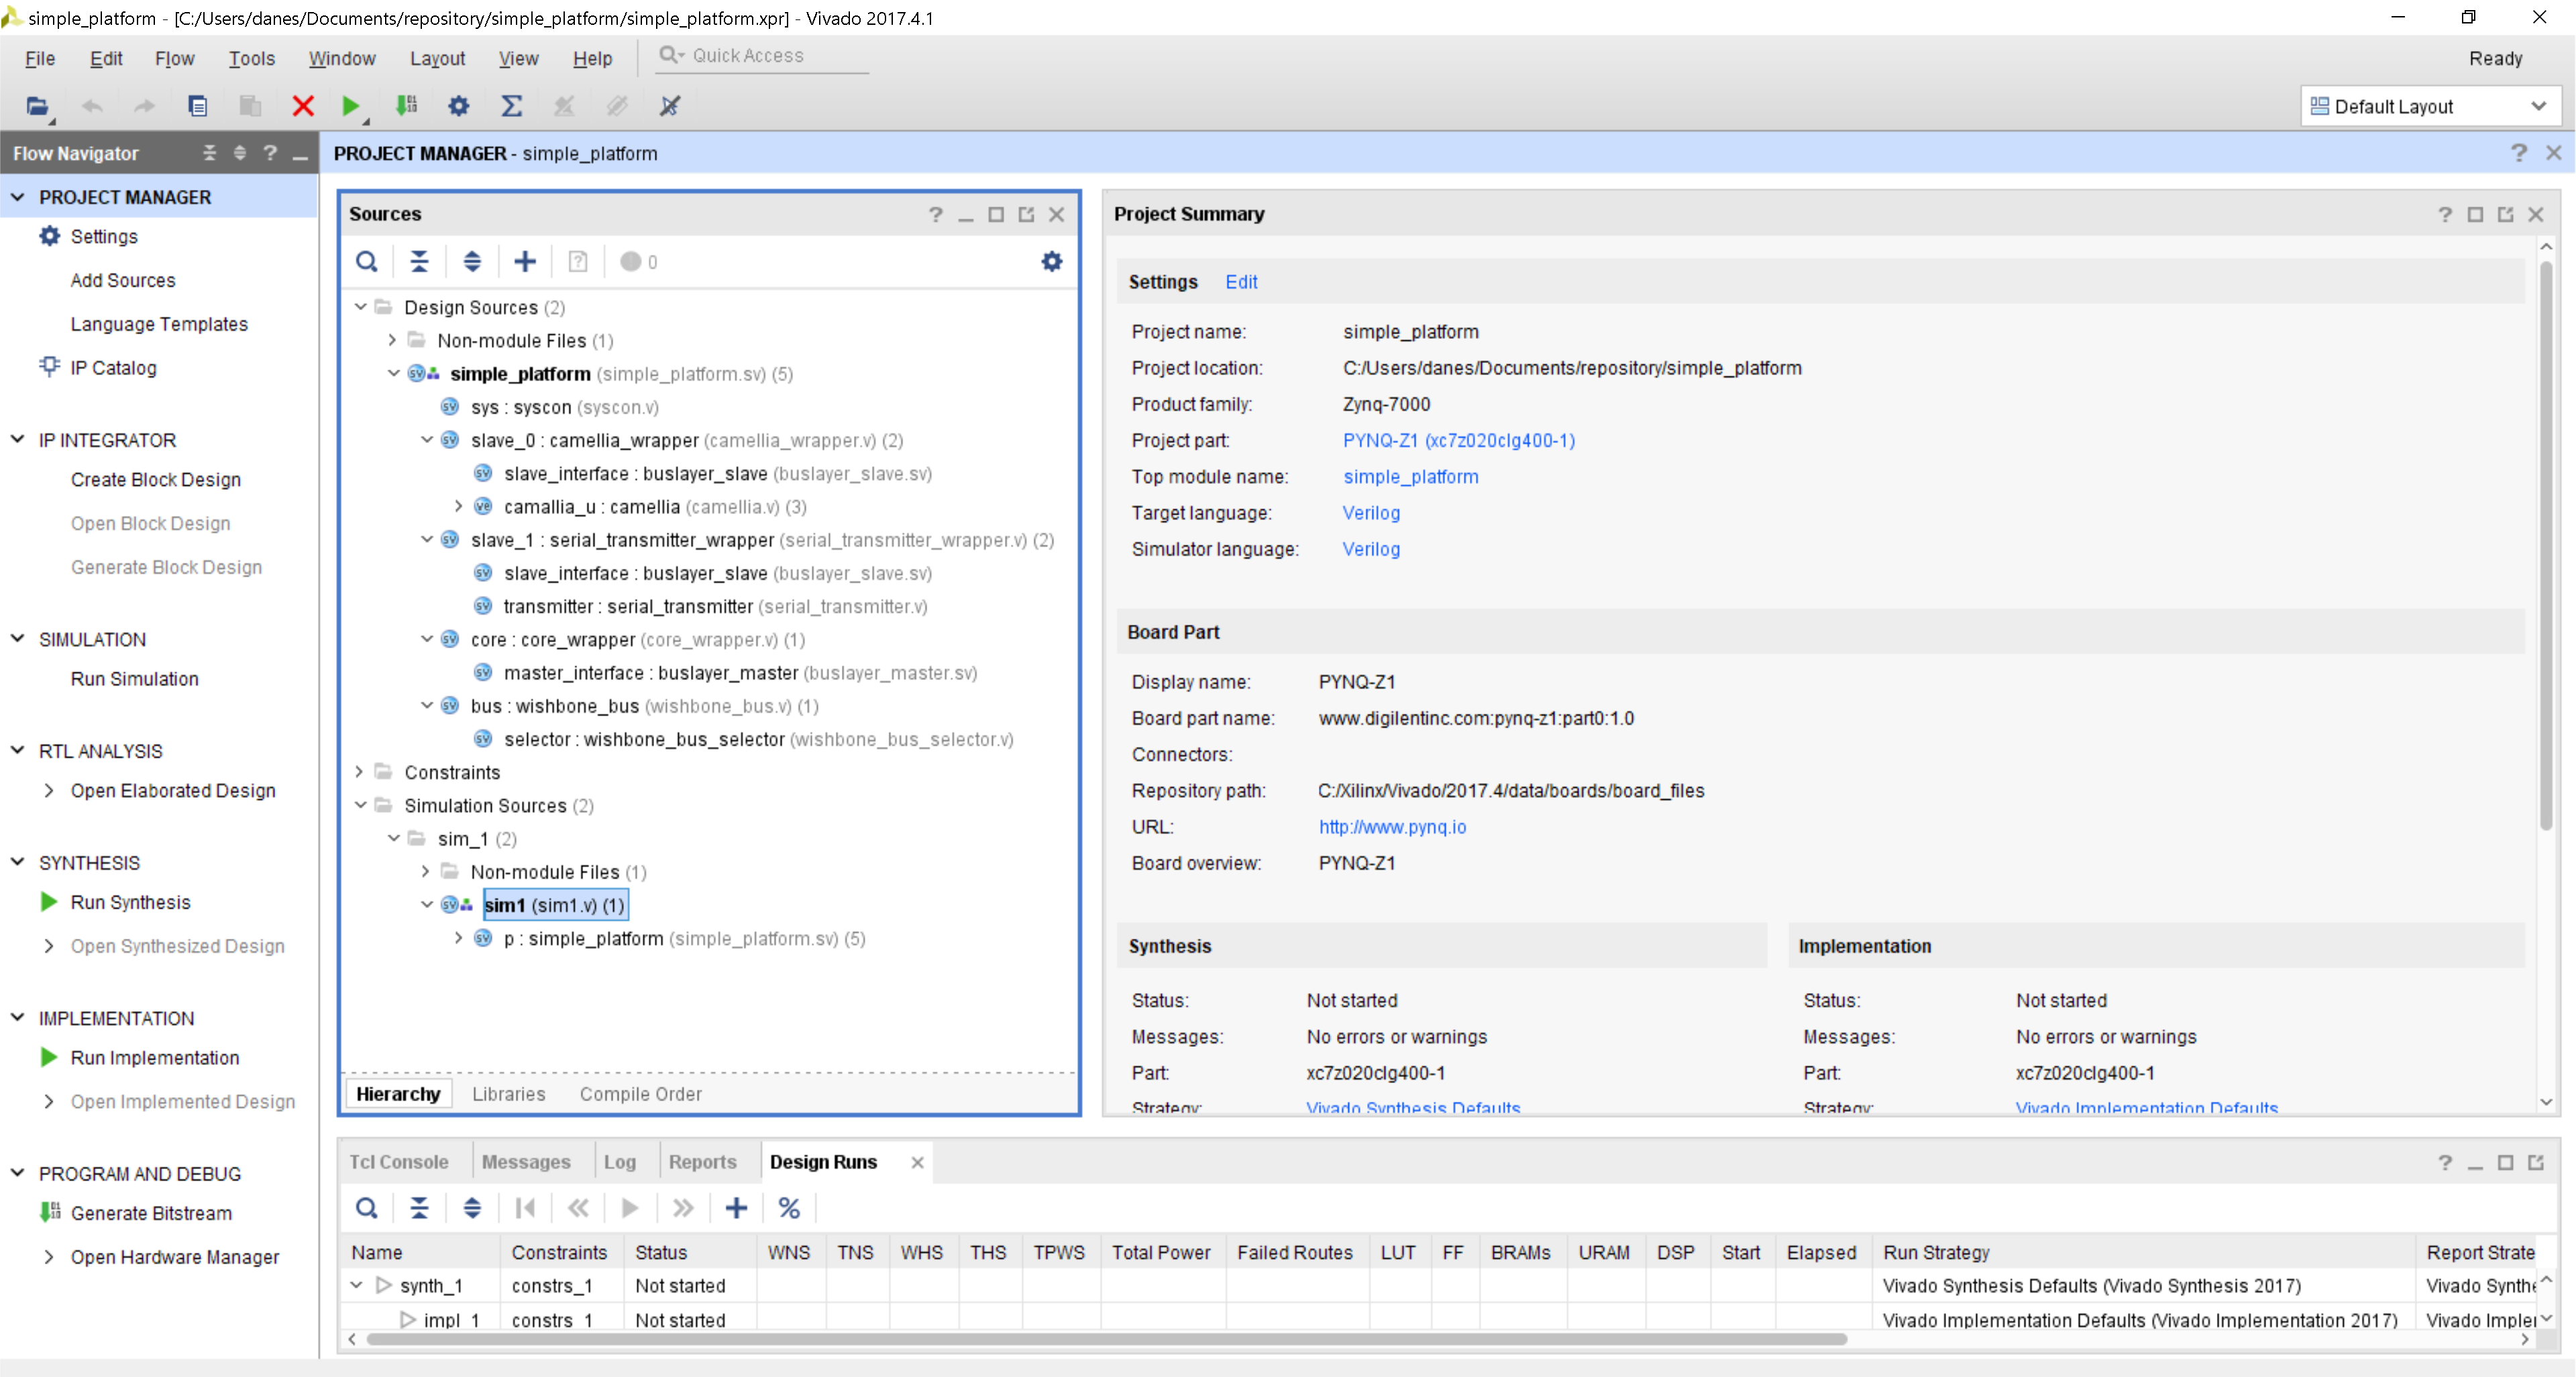
\includegraphics[width=0.9\columnwidth]{figures/vivado_sp.png}
\end{figure}

\end{frame}
%----------------------------------------------------------------------------------

%==================================================================================
\begin{frame}
\frametitle{EDA tools}

How to download EDA tools:

\begin{block}{}
\begin{enumerate}
\item
scp esd-student@esd-srv01.scienze.univr.it:/tmp/esdlab.tar.gz\\
(password: esd-student)
\item
tar -xvf esdlab.tar.gz
\item
cd esdlab
\item
source start\_eda.bash
\end{enumerate}
\end{block}

\end{frame}
%----------------------------------------------------------------------------------


%==================================================================================
\begin{frame}

\frametitle{Makefile menu}
How to open the Makefile menu (terminal):
\begin{block}{}
\begin{enumerate}
\item 
cd path2/sse-verifica/simple-platform/questa.simulation
\item
make
\end{enumerate}
\end{block}

\end{frame}
%----------------------------------------------------------------------------------


%==================================================================================
\begin{frame}

\frametitle{Makefile menu}
Once started, the following menu should appear on the terminal

\begin{figure}
\centering
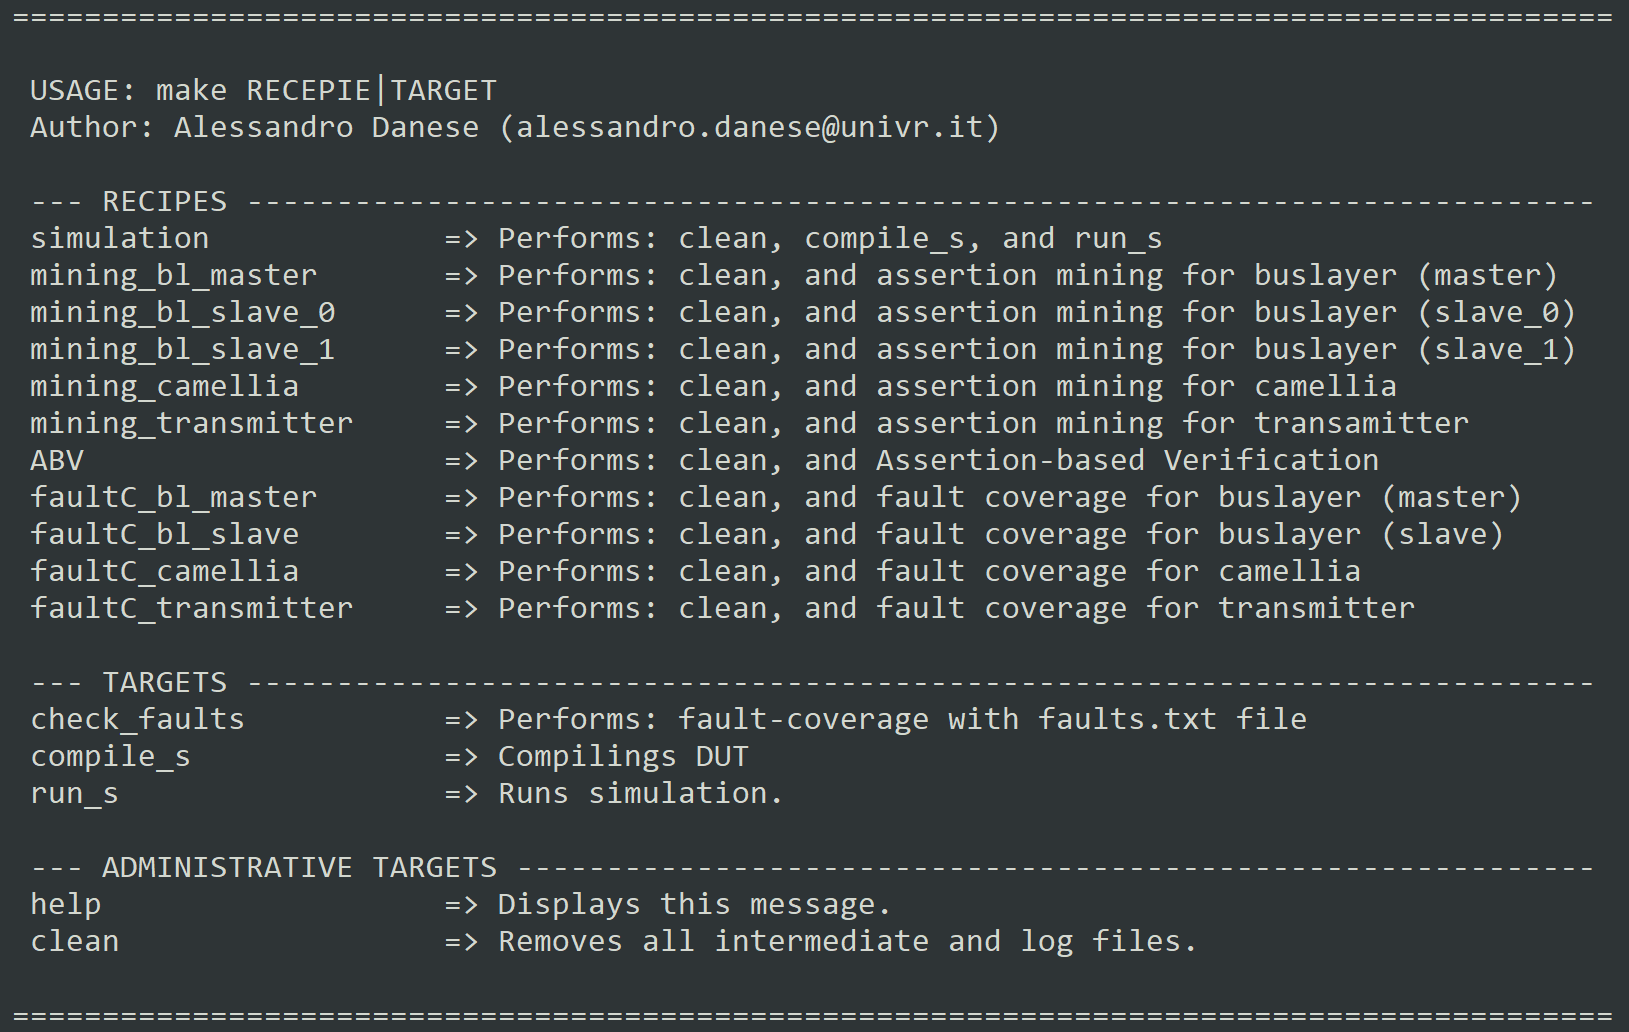
\includegraphics[width=0.9\columnwidth]{figures/makefile_menu.png}
\end{figure}
\end{frame}
%----------------------------------------------------------------------------------

%==================================================================================
\begin{frame}

\frametitle{Force}

The command force is a directive requiring the hardware simulator to force a value 
in a register/signal/port.

\begin{figure}
	\centering
	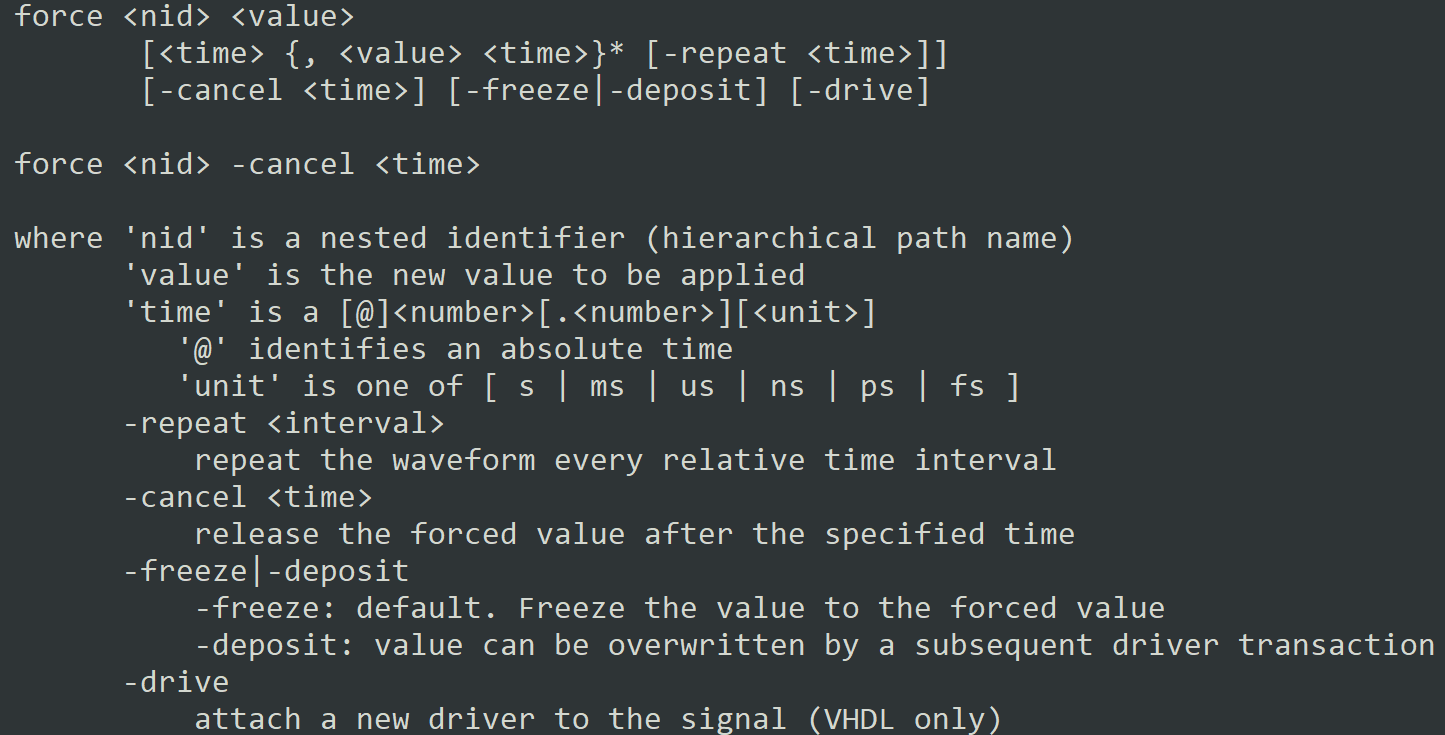
\includegraphics[width=0.9\columnwidth]{figures/force_cmd.png}
\end{figure}

\end{frame}
%----------------------------------------------------------------------------------

%==================================================================================
\begin{frame}

\frametitle{Example}

Forcing the bit input EN of camellia
\begin{itemize}
\item 
sim1.p.slave\_0.camallia\_u.EN 1'b0
\item
sim1.p.slave\_0.camallia\_u.EN 1'b1
\end{itemize}

Forcing the third bit of data input array of Transmitter
\begin{itemize}
\item 
sim1.p.slave\_1.transmitter.data(2) 1'b0
\item
sim1.p.slave\_1.transmitter.data(2) 1'b1
\end{itemize}

\end{frame}
%----------------------------------------------------------------------------------

%==================================================================================
\begin{frame}

\frametitle{Fault coverage}

How to perform fault coverage with the simple platform.
\begin{block}{Example transmitter}
	\begin{enumerate}
		\item 
		cd sse\_lesson1/questa.simulation
		\item
		make faultC\_transmitter
	\end{enumerate}
\end{block}

The command \textit{make faultC\_transmitter} injects forces to 
simulate stuck-at faults. The generated file coverage.txt reports the assertions 
failed for each injected fault.

\end{frame}
%----------------------------------------------------------------------------------

%==================================================================================
\begin{frame}

\frametitle{Exercise - 1}

\begin{enumerate}
	\item 
	Define a set of fault locations for the components transmitter.
	\item
	Define a set of assertions for the component transmitter.
	\item
	Run a fault coverage analysis to check if all injected faults are covered.
	\item
	Repeat steps 2 and 3 until all injected faults are covered by
	at least an assertion.
	
\end{enumerate}

  
\end{frame}
%----------------------------------------------------------------------------------

%%==================================================================================
%\begin{frame}
%
%\frametitle{Exercise - 2}
%
%Define a set of fault locations for the components buslayer\_master, and buslayer\_slave.\\~\\
%
%For each component, define a set of PSL properties such that any fault is covered
%by at least a property.
%
%\end{frame}
%%----------------------------------------------------------------------------------


%\begin{frame}
%\frametitle{Sample frame title}
%
%In this slide, some important text will be
%\alert{highlighted} beause it's important.
%Please, don't abuse it.
%
%\begin{block}{Remark}
%	Sample text
%\end{block}
%
%\begin{alertblock}{Important theorem}
%	Sample text in red box
%\end{alertblock}
%
%\begin{examples}
%	Sample text in green box. "Examples" is fixed as block title.
%\end{examples}
%\end{frame}

\end{document}